\section{結果}
開発したmy\_helpからhikiへの自動変換を可能にするmy\_help2hiki
のコマンドと使用法,それぞれのコードについて詳述する.
また,my\_help2hikiによる利点についても記述する.

\subsection{使用法,コマンド}
my\_helpからhikiに変換するときのコマンドと使用法は以下の通りである.
\begin{itemize}
\item TARGET --push : 作成したメモ(TARGET)をサーバに送る
\end{itemize}  
\begin{itemize}
\item my\_help --hiki : 作成したメモをhiki形式に変換し,wikiで表示できるようにする.
\end{itemize}

\subsection{TARGET --push のコードの詳述}
TARGET --pushのコードについて詳述する.
\begin{figure}[htbp]\begin{center}
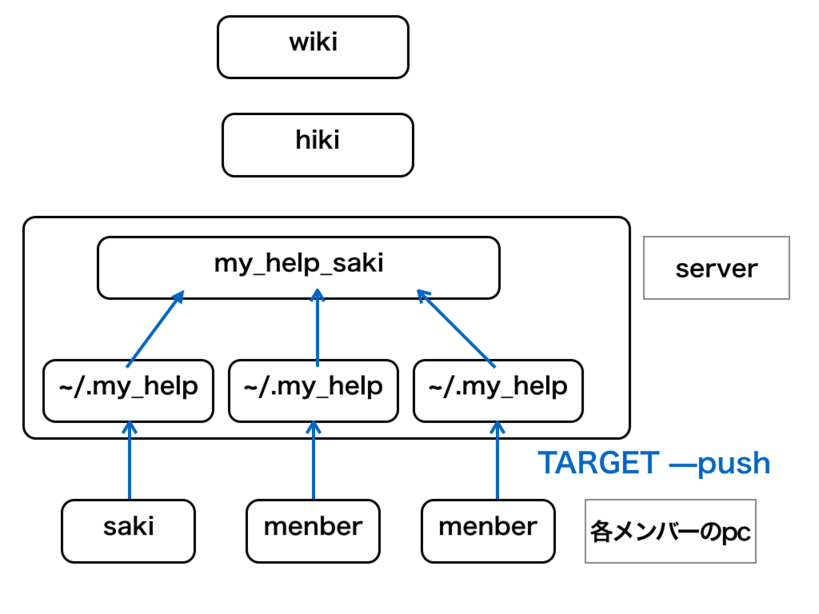
\includegraphics[width=6cm,bb=100 100 600 700]{my_help2hiki_saki.012.png}
\caption{TARGET --push}
\label{default}\end{center}\end{figure}

コードの中身は以下の通りである.
\begin{lstlisting}[style=,basicstyle={\scriptsize\ttfamily}]
    def push
      p "push my_todo"
      data_dir = File.join(ENV['HOME'],'.my_help')
      FileUtils.cd(data_dir)
      system "pwd"
      system "rm -rf ~/.my_help/*.yml~"
      system "scp -r ~/.my_help saki@nishitani0:~"
      system "ssh saki@nishitani0 ls ~/.my_help" 
    end
\end{lstlisting}
コードの詳細を記述する.
\begin{itemize}
\item 3,4行目
\end{itemize}
\begin{description}
\item my\_helpでは,作成したメモが.my\_helpのディレクトリに自動的に追加されるので,
ディレクトリを.my\_helpに移動する.
\end{description}
\begin{itemize}
\item 6行目
\end{itemize}
\begin{description}
\item .my\_helpにメモが追加されるとき,yaml形式のファイルで保存される.
メモを更新すると,一つ前に保存したファイルは*.yml~というファイル名
でバックアップとして残される.
\textbf{rm -rf}で不必要なファイルは削除し,サーバにコピーするときのデータ量を減らしている.
\end{description}

\begin{itemize}
\item 7行目
\end{itemize}
\begin{description}
\item
\textbf{scp -r ~/[directory名] [server名]}
のコマンドによってserverにssh接続を行い,directoryをserverにコピーする.
-rはディレクトリ全体をコピーすることを示している.
西谷研究室で利用しているnishitani0というサーバにコピーしている.
\end{description}

\begin{itemize}
\item 8行目
\end{itemize}
\begin{description}
\item nishitani0にssh接続し.my\_helpの中身を書き出して,
コピーができているかコマンドを実行した時に確認が行えるようにしている.
\end{description}

\newpage

\subsection{my\_help --hiki のコードの詳述}
my\_help --hikのコードについて詳述する.

\begin{figure}[htbp]\begin{center}
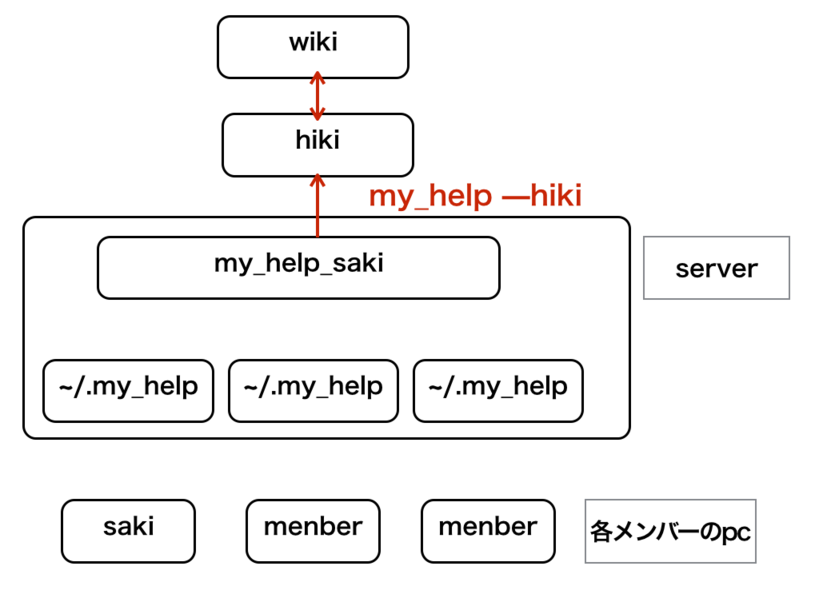
\includegraphics[width=6cm,bb=100 100 600 800]{my_help2hiki_saki.013.png}
\caption{my\_help2hiki}
\label{default}\end{center}\end{figure}

コードの中身は以下の通りである.
\begin{quote}\begin{verbatim}
def hiki
   p 'my_help2hiki'
   system "emacs_help --to_hiki > ~/Sites/hiki-1.0/data/text/emacs_help_saki"
   system "my_todo --to_hiki > ~/Sites/hiki-1.0/data/text/my_todo_saki"
   system "ssh_help --to_hiki > ~/Sites/hiki-1.0/data/text/ssh_help_saki"
   system "open -a safari 'http://localhost/~saki/hiki-1.0/?FrontPage'"
end
\end{verbatim}\end{quote}
\newpage
コードの詳細について記述する.
\begin{itemize}
\item 2-4行目
\end{itemize}
\begin{description}
\item my\_helpには,\textbf{TARGET --to\_hiki}というコマンドがあり,これによって
yaml形式で保存されているメモをhiki形式で書き出すことができる.
この --to\_hiki のコマンドを使ってhiki形式にしたものを,wikiで表示することのできる
フォルダである\textbf{~/Sites/hiki-1.0/data/text/}に入れることで,wikiでの表示を可能にしている.
emacs\_help,my\_todo,ssh\_helpは全て私のmy\_helpに入っているメモ.
\end{description}

\begin{itemize}
\item 5行目
\end{itemize}
\begin{description}
\item wikiのページである,図6に示したFrontPageを表示するコマンド.
これによりメモが更新されているのをすぐに確認することができる.
FrontPageは以下のようになっている.
\end{description}
\begin{quote}\begin{verbatim}
!saki's help
*[[ssh_help_saki]]
*[[my_todo_saki]]
*[[emacs_help_saki]]
\end{verbatim}\end{quote}
\begin{description}
\item 先頭に\textbf{!}をつけることで1行目のsaki's helpを見出しにし,
2~4行目は\textbf{*}によって箇条書き,角括弧でリンクになっている.
\end{description}

\begin{figure}[htbp]\begin{center}
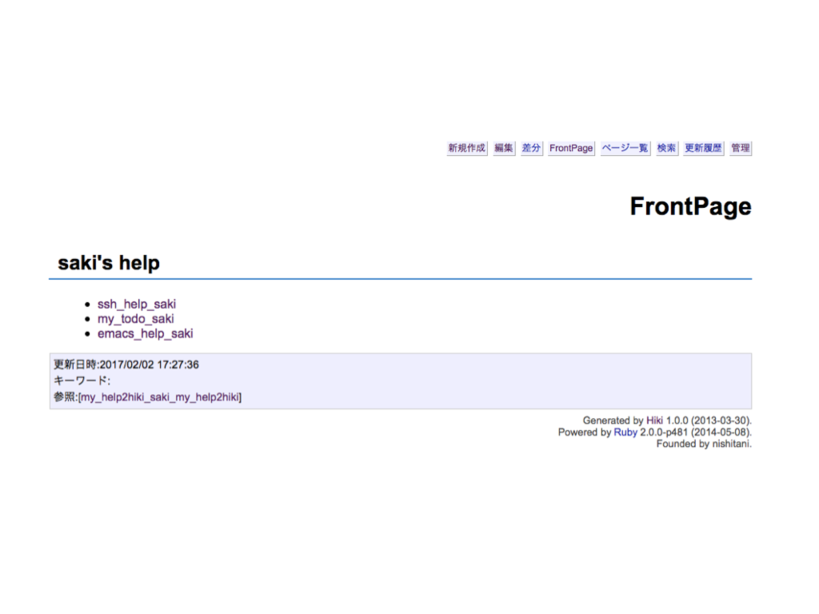
\includegraphics[clip,width=6cm,bb=100 100 600 550]{my_help2hiki_saki.002.png}
\caption{コマンドを実行したときに開くFrontPage }
\label{default}\end{center}\end{figure}

\subsection{my\_help2hikiによる利点}
my\_help2hikiによる利点について述べる.

\begin{quote}\begin{verbatim}
/Users/saki% my_help --list
Specific help file:
  emacs_help	:emacsのキーバインド
  memo_help	:ヘルプのサンプル雛形
  my_todo	:my_todo
  ssh_help	:sshのhelp
\end{verbatim}\end{quote}

これは私のmy\_helpの中身を書き出している.
下がemacs\_helpの中身である.

\begin{quote}\begin{verbatim}
/Users/saki% emacs_help --all
emacsのキーバインド

特殊キー操作
  c-f, controlキーを押しながら    'f'
  M-f, escキーを押した後一度離して'f'
    操作の中断c-g, 操作の取り消し(Undo) c-x u
     cc by Shigeto R. Nishitani, 2016
+emacsのキーバインド:
+
特殊キー操作
+  c-f, controlキーを押しながら    'f'
+  M-f, escキーを押した後一度離して'f'
+    操作の中断c-g, 操作の取り消し(Undo) c-x u
+     cc by Shigeto R. Nishitani, 2016:
---
-カーソル移動cursor:
+c-f, move Forwrard,    前or右へ
+c-b, move Backwrard,   後or左へ
+c-a, go Ahead of line, 行頭へ
+c-e, go End of line,   行末へ
+c-n, move Next line,   次行へ
+c-p, move Previous line, 前行へ
---
---
-ページ移動page:
+c-v, move Vertical,          次のページへ
+M-v, move reversive Vertical,前のページへ
+c-l, centerise Line,       現在行を中心に
+M-<, move Top of file,    ファイルの先頭へ
+M->, move Bottom of file, ファイルの最後尾へ
---
---
-ファイル操作file:
+c-x c-f, Find file, ファイルを開く
+c-x c-s, Save file, ファイルを保存
+c-x c-w, Write file NAME, ファイルを別名で書き込む
---
---
-編集操作edit:
+c-d, Delete char, 一字削除
+c-k, Kill line,   一行抹消,カット
+c-y, Yank,        ペースト
+c-w, Kill region, 領域抹消,カット
+領域選択は,先頭or最後尾でc-spaceした後,最後尾or先頭へカーソル移動
+c-s, forward incremental Search WORD, 前へWORDを検索
+c-r, Reverse incremental search WORD, 後へWORDを検索
+M-x query-replace WORD1 <ret> WORD2:対話的置換(y or nで可否選択)
---
---
-ウィンドウ操作window:
+c-x 2, 2 windows, 二つに分割
+c-x 1, 1 windows, 一つに戻す
+c-x 3, 3rd window sep,縦線分割
+c-x o, Other windows, 次の画面へ移動
---
---
-バッファー操作buffer(すでにopenしてemacsにバッファーされたfile):
+c-x b, show Buffer,   バッファのリスト
+c-x c-b, next Buffer, 次のバッファへ移動
---
---
-終了操作quit:
+c-x c-c, Quit emacs, ファイルを保存して終了
+c-z, suspend emacs,  一時停止,fgで復活
\end{verbatim}\end{quote}

このように各学生のメモを何種類も作成できるが,自分のパソコンでしか見ることができなかった.
本研究によるmy\_help2hikiを使うことで,図6のようにmy\_helpをwikiで表示可能になり,
各学生のメモを研究室内で共有することができるようになる.
今までも作成したメモをhikiに変換し,wikiで表示することは可能であったが,
メモを更新するたびにその作業をすることは手間がかかる.
本研究で開発したmy\_help2hikiを用いることで手間が省けるので,研究室内での
ナレッジマネジメントが促進されることが期待される.